\section{亚线性复杂度PIR的基本构造}
我们基于现有的亚线性PIR方案\cite{EC:CorKog20, C:LazPap23}构建可验证PIR,对这些方案的认识有助于理解本文提出的新方案。我们从如图\ref{fig:CK20}所示的两服务器PIR方案起步,讨论如何修正该协议的局限性。该协议是一个离线-在线PIR方案,我们使用$\hintserver$ 与 $\queryserver$ 两个记号来区分协议中涉及到的两台服务器。这些记号是根据两台服务器的功能定义的:

\subsection{构造方案}

\noindent \textbf{离线阶段:}
\begin{itemize}
\item \textbf{Setup:} 客户端$\client$ 生成$\hintcount$ 组集合$\setkey_j, j\in[\hintcount]$。每个集合包含$\setsize$个在范围[$\dbsize$]内的随机索引。
\item \textbf{Hint:}$\client$将这些集合转发给$Hint$服务器$\hintserver$。$\hintserver$计算这些集合对应数据库中记录的和,表示为$\hint_j \coloneqq \sum_{k\in \setkey_j} \db_k, j \in [\hintcount]$。$\client$存储这些集合及其对应的记录之和作为校验值。
\end{itemize}

\noindent \textbf{在线阶段:}
\begin{itemize}
\item \textbf{Query:}$\client$首先找出一个包含目标索引$\dbidx$的集合$\setkey_\hintidx$,并从该集合中去掉$\dbidx$,$\queryquery \coloneqq \setkey_\hintidx \setminus \{\dbidx\}$。此外,$\client$生成一个包含索引$\dbidx$的新集合$\setkey'$,并令$\hintquery \coloneqq \setkey' \setminus \{\dbidx\}$。$\client$将集合$\hintquery$发送给$Hint$服务器$\hintserver$,将$\queryquery$发送给$Query$服务器$\queryserver$。
\item \textbf{Answer:} 收到这些集合后,服务器分别为两个集合计算校验值,$\queryanswer\coloneqq \sum_{j\in \queryquery}\db_j$,$\hintanswer\coloneqq \sum_{j\in \hintquery}\db_j$,将这些校验值发送给$\client$。
\item \textbf{Reconstruct:}$\client$ 计算出所需的记录:$\db_\dbidx \coloneqq \hint_\hintidx - \queryanswer$。
\item \textbf{Refresh:}$\client$ 更新$Hint$: $\setkey_\hintidx \coloneqq \setkey'$,$\hint_\hintidx \coloneqq \hintanswer+\db_\dbidx$。
\end{itemize}


\subsection{基本构造的缺陷}
不妨先假设客户端生成的集合足够多,在$Query$阶段总能找到包含目标索引的集合。在此前提下,客户端总能得到想要查询的记录$\db_\dbidx$,该协议的正确性显而易见。然而,该协议存在三个关键问题:

\begin{enumerate}
\item \textbf{低效的集合隶属测试:} 搜索包含查询索引$\dbidx$的集合$\setkey_t$的过程计算量很大。客户端需要遍历所有集合,同时遍历集合中的元素已确定某个索引是否隶属于这个集合。尽管可以通过排序和二分查找进行优化,但它仍然需要$O(\sqrt{\dbsize}\log \dbsize)$的在线计算复杂度。
\item \textbf{低下的空间和通信效率:} 对客户端来说,以明文形式生成、存储和发送这些集合的效率低下,客户端完成协议时需要$O(\dbsize)$的存储和离线通信复杂度。粗略估计,为了确保正确性,客户端需要大约$\hintcount = O(\lambda\sqrt{\dbsize})$个集合,每个集合的大小为$\setsize = \sqrt{\dbsize}$。相应的存储和离线通信复杂度为$O(\lambda\dbsize)$。
\item \textbf{有缺陷的隐私性:} 集合$\queryquery$和$\hintquery$不可能包含查询的索引$\dbidx$。从信息论角度来看,这泄露了大约$1/(\sqrt{\dbsize}\ln 2)$比特$\dbidx$的信息。
\end{enumerate}

\subsection{虚设查询及其引入的新问题}
在现有工作中,研究者已经提出了多种方法来解决上述问题。例如,TreePIR \cite{C:LazPap23} 利用了一种称为弱可穿孔伪随机函数(Weakly Puncturable Pseudorandom Function)的原语,并引入了一种新的亚线性PIR构造。 Piano \cite{Piano} 提出了一个类似的算法,称为$PossibleParities$。然而,当尝试向这些协议中引入可验证性时,这些方案遇到了类似的困境,本文总结为“虚设查询”。

\begin{figure}
    \centering
    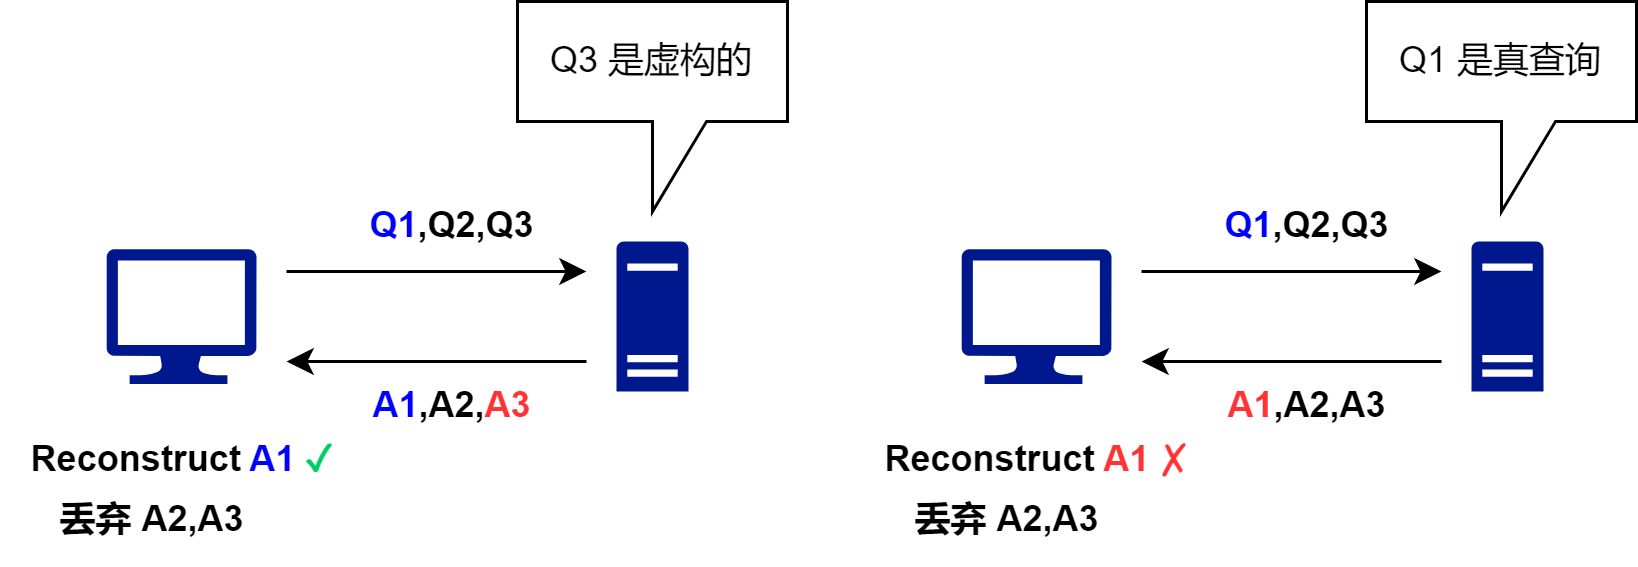
\includegraphics[width=1\linewidth]{figure/dummy.png}
    \caption{关于虚设查询的图示}
    \label{fig:dummy}
\end{figure}

这些虚设查询是随机生成的假查询,其目的是与真实查询相混淆。在这些方案中,客户端发送的单个查询会泄露关于查询索引$\dbidx$的信息给服务器。通过真实查询与虚设查询的组合,协议才得以隐藏索引$\dbidx$。服务器无法区分虚设查询与真实查询,所以会对虚设查询同样作出回应,但客户端会忽略对虚设查询的回应。

在半诚实环境下,这些方案的隐私性依赖于服务器无法区分真实查询和虚设查询。然而,在可验证PIR的设定下,选择失败攻击会使虚设查询失效。这是由于在验证过程中,客户端只能在真实查询的答案被篡改时拒绝服务器的响应。客户端没有在离线阶段获得这些虚设查询的校验信息,因此无法计算和验证虚设查询的答案。在这种情况下,服务器可以选择性地篡改其中数个答案,通过客户端的验证结果推断出被篡改的答案是否对应了真实查询。这一漏洞使得恶意服务器有可能得知客户端正在查询的索引,导致我们无法在现有亚线性PIR方案中引入可验证性。图\ref{fig:dummy}展示了该问题的一个示例。客户端向服务器发送了3个查询,其中第一个查询是真实查询,另外两个是虚设查询。由于客户端只能拒绝对真实查询的错误答案,接受对虚设查询的错误答案,因此服务器可以操纵答案,从客户端的验证结果中推断信息。除了隐私问题外,计算虚设查询的答案也增加了在线计算的成本。为了提高效率,应对选择失败攻击,我们的方案\textbf{消除了虚设查询}。

